\documentclass[twoside]{article}
\usepackage{format/aistats2e}
\usepackage{amssymb,amsmath,amsthm}
\usepackage{graphicx}
\usepackage{preamble}
\usepackage{natbib}
\usepackage{hyperref}
\usepackage{color}
\definecolor{mydarkblue}{rgb}{0,0.08,0.45}
\hypersetup{ %
    pdftitle={},
    pdfauthor={},
    pdfsubject={},
    pdfkeywords={},
    pdfborder=0 0 0,
    pdfpagemode=UseNone,
    colorlinks=true,
    linkcolor=mydarkblue,
    citecolor=mydarkblue,
    filecolor=mydarkblue,
    urlcolor=mydarkblue,
    pdfview=FitH}
    
    
% If your paper is accepted, change the options for the package
% aistats2e as follows:
%
%\usepackage[accepted]{aistats2e}
%
% This option will print headings for the title of your paper and
% headings for the authors names, plus a copyright note at the end of
% the first column of the first page.


\begin{document}

% If your paper is accepted and the title of your paper is very long,
% the style will print as headings an error message. Use the following
% command to supply a shorter title of your paper so that it can be
% used as headings.
%
%\runningtitle{I use this title instead because the last one was very long}

% If your paper is accepted and the number of authors is large, the
% style will print as headings an error message. Use the following
% command to supply a shorter version of the authors names so that
% they can be used as headings (for example, use only the surnames)
%
%\runningauthor{Surname 1, Surname 2, Surname 3, ...., Surname n}

\twocolumn[

\aistatstitle{Structure Search in Gaussian Process Models}

\aistatsauthor{ Anonymous Author 1 \And Anonymous Author 2 \And Anonymous Author 3 }

\aistatsaddress{ Unknown Institution 1 \And Unknown Institution 2 \And Unknown Institution 3 } ]

\begin{abstract}
Gaussian process (GP) models are used widely and successfully.  However, their effictiveness depends critically on choosing an appropriate family of kernels.  This aspect of GP modeling has been sorely underdeveloped.  In this paper, we introduce a procedure for automatically and efficiently searching through a large space of GP models.
\end{abstract}

\section{INTRODUCTION}

Similar searches over large model classes have been succesfully used in machine vision [cite Cox + Pinto].  In general, learning the model class from data seems superior proposing the model beforehand.  In high dimensional problems, it is also hard for a practitioner to propose an appropriate model even after examining a dataset closely.  Choosing a kernel family is also a stumbling block for non-experts who wish to use Gaussian Process models.

\section{GP STRUCTURE}

[Standard GP intro \cite{rasmussen38gaussian}]

\section{MODEL-BASED SEARCH OVER MODELS}

Bayesian optimization for hyper-parameter search: \cite{snoek2012practical}

\subsection{Bayesian Optimization}

\subsection{A Kernel between kernels}

Hyperkernels \cite{ong2002hyperkernels}

\section{EXPERIMENTS}

\subsection{Maunal Loa Atmoshperic Carbon Dioxide}

As an example of a GP modeling problem where choosing an appropriate structure is critical, we revisit a dataset explored in \cite{rasmussen38gaussian}, pages 120-126, where a kernel was hand-tailored to fit a GP model to the dataset.

\begin{figure}
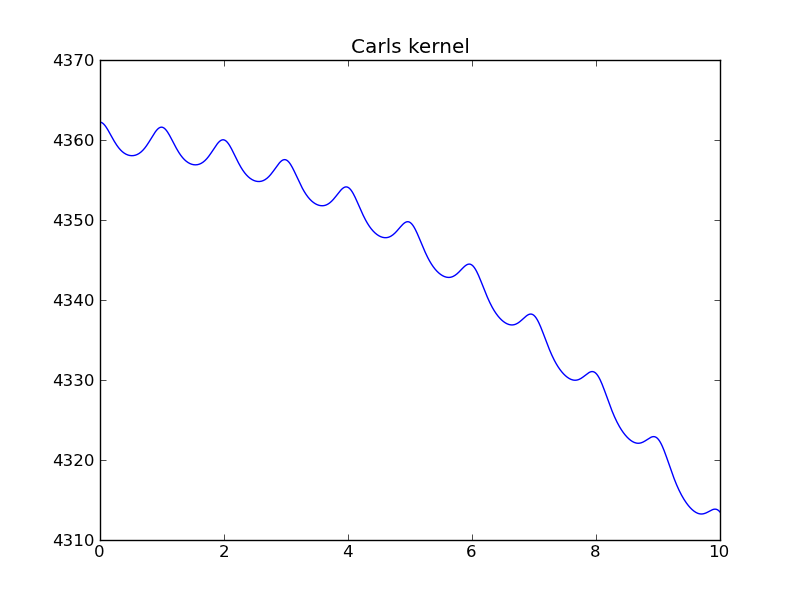
\includegraphics[width=\columnwidth]{../figures/carls_kernel}
\caption{Carl's kernel function on the Mauna dataset.}
\end{figure}

\begin{figure}
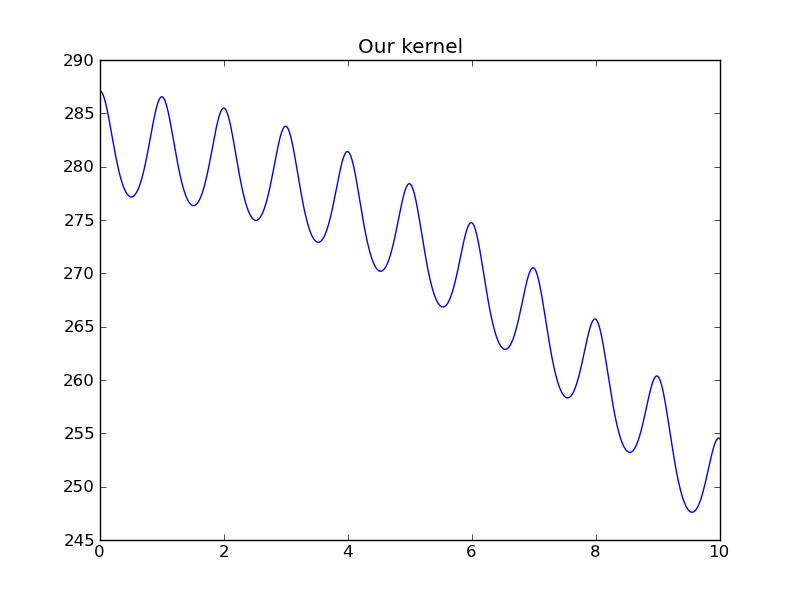
\includegraphics[width=\columnwidth]{../figures/our_kernel}
\caption{Our best kernel function on the Mauna dataset.}
\end{figure}

\begin{figure}[h]
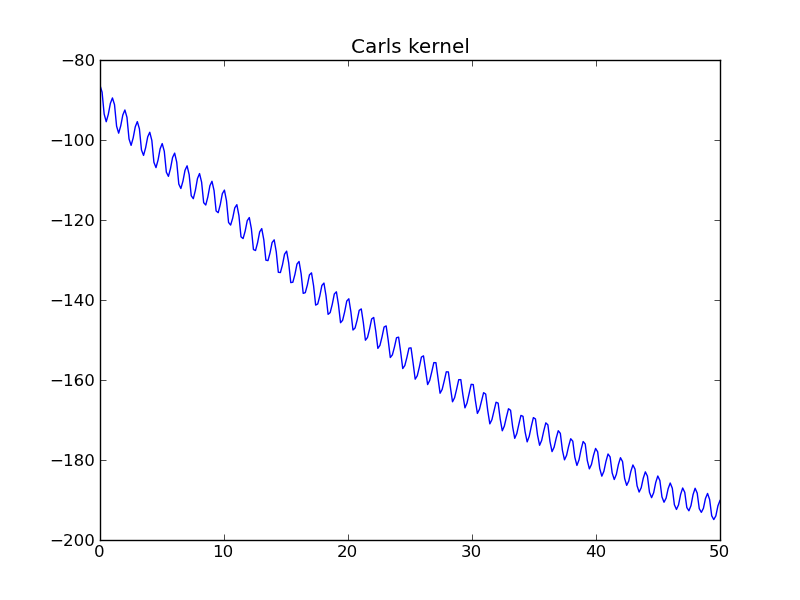
\includegraphics[width=\columnwidth]{../figures/carls_kernel_draw1}
\caption{A draw from Carl's kernel.}
\end{figure}

\begin{figure}[h]
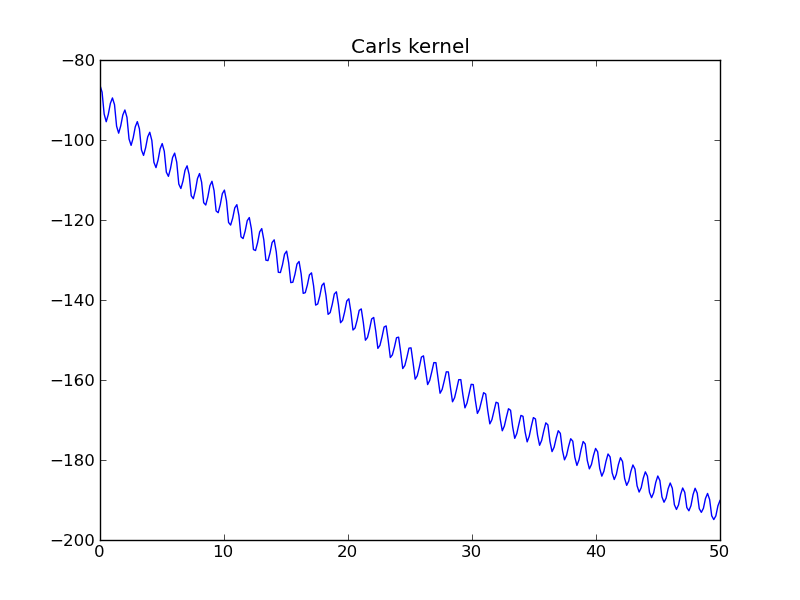
\includegraphics[width=\columnwidth]{../figures/carls_kernel_draw1}
\caption{Another draw from Carl's kernel.}
\end{figure}

\begin{figure}[h]
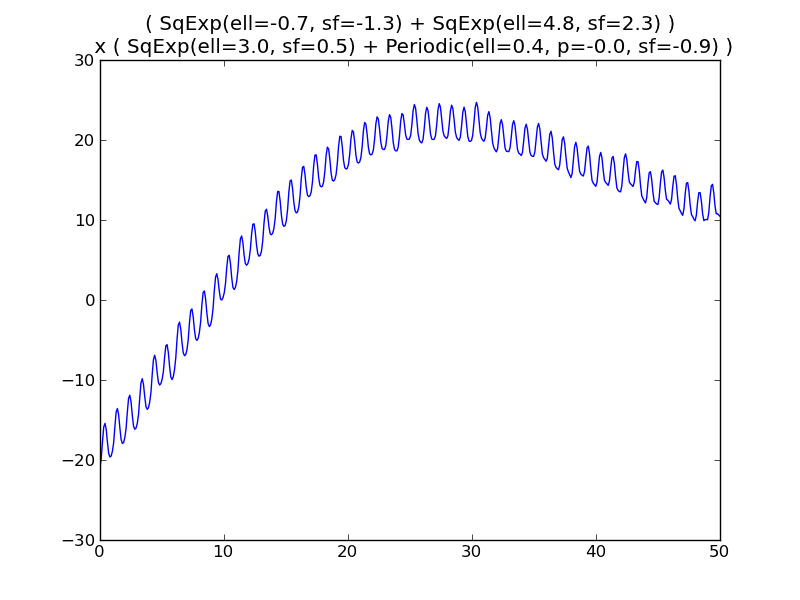
\includegraphics[width=\columnwidth]{../figures/mauna_prior_draw_best_cov_v3}
\caption{Another draw from our kernel.}
\end{figure}

\begin{figure}[h]
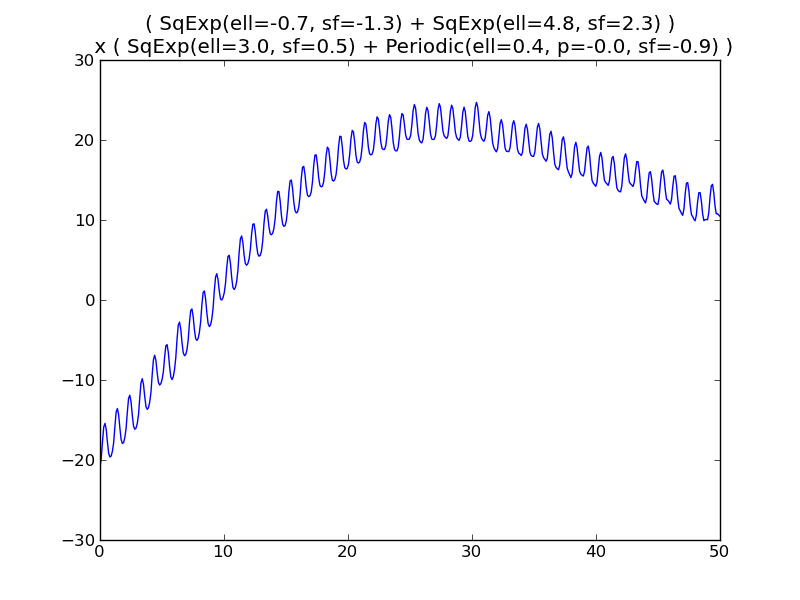
\includegraphics[width=\columnwidth]{../figures/mauna_prior_draw_best_cov_v3}
\caption{Another draw from our kernel.}
\end{figure}

\subsection{Load forecasting}

\subsection{Synthetic experiments}

\subsection{Real datasets}

\section{RELATED WORK}

Compositional Model search for unsupervsied learning: \cite{grosse2012exploiting}

Additive Gaussian Processes \cite{duvenaud2011additive11}

Hyperkernels \cite{ong2002hyperkernels}

\subsection{Genetic Searches}

Evolving kernel functions for SVMs by genetic programming: \cite{diosan2007evolving}

A Genetic Programming based kernel construction and optimization method for Relevance Vector Machines: \cite{bing2010gp}

\subsection{Equation Learning}

Equation discovery with ecological applications \cite{dzeroski1999equation}

%Discovering admissible model equations from observed data based on scale-types and identity constraints \cite{washio1999discovering}



\section{DISCUSSION}

Machine learning can be more data-driven, analogous to the high-thoughput approaches being used in biology. 


\section{CONCLUSION}


\subsubsection*{Acknowledgements}


\bibliographystyle{format/icml2013}
\bibliography{gpss}

\end{document}
